\documentclass[twocolumn]{svjour3}       % onecolumn (second format)
\usepackage{graphicx}
\usepackage{tabularx}
\usepackage{url}
\usepackage[utf8]{inputenc}
\usepackage{listings}
\lstset{ 
  basicstyle=\footnotesize,
  frame=single,              
  breaklines=true,               
  breakatwhitespace=false,  
  title=\lstname
}
\usepackage[acronym, nonumberlist, style=super]{glossaries}
\bibliographystyle{plain}    % Springer style is completely broken 
\journalname{Journal of Grid Computing}
\begin{document}

\title{Towards Standardized Job Submission and Control in Infrastructure Clouds}
\author{Peter Tr\"oger \and Andre Merzky}
\institute{Peter Tr\"oger \at
              Hasso Plattner Institute, University of Potsdam \\
              \email{peter.troeger@hpi.uni-potsdam.de}          
              \and
              Andre Merzky \\
              CCT, Louisiana State University \\
              \email{andre@merzky.net}
}

\date{Received: date / Accepted: date}

\maketitle

\newacronym{api}{API}{Application Programming Interface}
\newacronym{bes}{BES}{Basic Execution Service}
\newacronym{cdmi}{CDMI}{Cloud Data Management Interface}
\newacronym{dmtf}{DMTF}{Distributed Management Task Force}
\newacronym{dom}{DOM}{Document Object Model}
\newacronym{drmaa}{DRMAA}{Distributed Resource Management Application API}
\newacronym{drms}{DRMS}{Distributed Resource Management System}
\newacronym{drm}{DRM}{Distributed Resource Management}
\newacronym{gat}{GAT}{Grid Application Toolkit}
\newacronym{hpc}{HPC}{High Performance Computing}
\newacronym{idl}{IDL}{Interface Definition Language}
\newacronym{jcl}{JCL}{Job Control Language}
\newacronym{jsdl}{JSDL}{Job Submission Definition Language}
\newacronym{occi}{OCCI}{Open Cloud Computing Interface}
\newacronym{ogf}{OGF}{Open Grid Forum}
\newacronym{ovf}{OVF}{Open Virtualization Format}
\newacronym{saga}{SAGA}{Simple API for Grid Applications}
\newacronym{snia}{SNIA}{Storage Networking Industry Association}
\newacronym{wsrf}{WSRF}{Web Service Resource Framework}
\makeglossaries


\begin{abstract}
The submission and management of computational jobs in a distributed batch processing system is a traditional part of utility computing environments. End users and developers of domain-specific software abstractions often have to deal with the heterogeneity of such systems. This lead to a number of application programming interface and job description standards in the past, which are implemented and established for cluster and grid systems.

With the recent rise of cloud computing as new utility computing paradigm, the standardized access to batch processing facilities operated on cloud resources becomes an important issue. Furthermore, the design of such a standard has to consider a tradeoff between feature completeness and the achievable level of interoperability. This article discusses this general challenge, and presents some existing standards with traditional cluster and grid computing background that may be applicable to cloud environments. We furthermore present the OCCI-DRMAA approach as one way of defining a standardized access to batch processing facilities hosted in a cloud. 
\end{abstract}

%keywords: cloud; IaaS; DRMS; DRMAA; OCCI; batch processing; job submission; job monitoring
\sloppy

\section{Introduction}
\label{intro}

Batch processing is a traditional approach in IT systems. It originated in the batched execution of punch cards on early computer systems, and helped to improve the throughput of computational job execution on very expensive IT resources. Many modern operating system concepts, such as supervisor mode versus user mode, have their foundation in these batch systems. 

 With the advent of cheap distributed hardware in the 80's, batch processing moved to distributed installations of collaborating computer systems, called \emph{clusters}. This lead to the development of cluster management systems for job scheduling, execution host management and monitoring. Typical examples for such systems are GridEngine, the Portable Batch System (PBS), Torque, LoadLeveler, or HTCondor. A cluster infrastructure maps incoming computational jobs to the available set of distributed resources. The largest user base for massively scaled cluster environments exists in the \gls{hpc} community, where the scalable execution of massively parallel jobs is the primary goal. For several decades, the \gls{hpc} community had a primary focus on locally distributed cluster systems, where parallel application instances are managed by a local \gls{drms} scheduler, for a set of nodes. Meanwhile, the federated usage of geographically distributed resources through a single interface became another important part of \gls{drms} operation -- this is the main usage mode for \emph{grid computing} environments, which is largely motivated by applications with large scientific computational and storage demands, such as the \emph{Large Hadron Collider} project. 

 Batch processing in itself is not only an \gls{hpc} concept -- IBM mainframe systems, for example, support a wide area of transaction-oriented applications with their \gls{jcl} description syntax and scheduler implementations. Another example are modern data-parallel execution frameworks for the map-reduce programming model, which implicitly organize job distribution and management for executed applications.

For each of these usage scenarios for a batch processing system, a common question is the design of interfaces to the \gls{drm} system functionality: how can they be developed so as to use as broad a range of infrastructure as possible, without vendor or middleware lock-in, yet with the flexibility and performance that is required. This question assumes greater significance in the distributed computing context, such as grids and clouds, where resource owners and users are more decoupled than for most other modes of computing.

One design perspective is the end user perspective, were humans (or their shell scripts) interact with the \gls{drm} system. Typical solutions motivated by that perspective are command-line tools and graphical user interfaces provided by the particular \gls{drm} framework. An alternative design perspective focuses more on programmatic access to the \gls{drm} system's functionality -- whenever the batch job submission is used by higher level software (e.g. meta-scheduling systems or domain-specific user interface implementations), that software controls the \gls{drm} system through some \gls{api}.

Whether the \gls{drm} system is controlled through user tools or through a product \gls{api}, it must be possible to describe job requirements in some format. This relates to the fact that batch processing is inherently tied to non-interactive jobs, where the request for execution is formulated as a set of job parameters. This includes properties such as the executable name and location, and hardware and operating system requirements. Such \emph{job description} is handed over to the \gls{drm} system for interpretation, scheduling and finally execution. 

As long as cluster systems were mainly used as organization-specific local resource, it was acceptable to realize job requirement descriptions and programmatic product access through vendor-specific solutions. With the increasing relevance of grid computing and it's federation aspect, it became more and more important to have more unified interfaces to resource management systems, as users were exposed to a multitude of system flavors within a single grid infrastructure. This lead to a number of standardization efforts, mainly in the \gls{ogf} standardization body. Different job description formats and interface approaches gained wide-spread acceptance, especially in the academic \gls{hpc} community. It is now widely and independently acknowledged that a uniform, simple and stable access layer is necessary (but not sufficient) to improve end user experience on distributed computing infrastructures.

With the established grid computing paradigm and the according standards being in place, a new utility computing paradigm arose around 2000 - \emph{cloud computing}. We refer to related articles for a discussion about the commonalities between grid and cloud computing~\cite{citemaster_9642}, but want to emphazise the fact that cloud computing is an industry-driven business model, where a provider offers one or more of the following service classes:

\begin{description}
\item[Infrastructure as a Service (IaaS)] - The service provider offers virtualized compute or storage resources as remotely accessible asset. Well-known examples for providers are Amazon EC2, Microsoft Azure, Rackspace Cloud, or Google Compute Engine. The offers often include auxilliary services such as virtual network switches or software bundles. 
\item[Platform as a Service (PaaS)] - The service provider offers an execution platform for software written by the customer. The platform provides automated application scalability and availability, as long as the customer software follows a particular programming model. Well-known examples for such offerings are the Google AppEngine or Heroku.
\item[Software as a Service (SaaS)] - The service provider operates remotely usable software that has tenant capabilities. Well-known examples are Microsoft Office 365, Salesforce or the Amazon Web Services. 
\end{description}

Even though the majority of sources declares these service classes as layered concepts, providers can operated and offer them independently: one example is the Google AppEngine offering, which does not fully rely on the IaaS offering by the same company.

\section{Motivation}

With the recent acceptance of the cloud computing paradigm as billing and management approach for federated resource usage, it became also interesting for the \gls{hpc} community. Several data centers, originally designed with a \emph{closed world assumption} in mind, already opened their resources to grid computing initiatives for external usage~\cite{unicore}. These stakeholders are now about to introduce cloud offerings for their resources, in order to maximize utilization and gain some revenue from the provisioning. A second relevant trend is the rise of \emph{Private Cloud} solutions, were organizations operate their own cloud infrastructure for the purpose of easier management and internal accounting~\cite{}. Due to both trends, the relevance of classical job submission is increasing for cloud computing infrastructures. 

With this article we want to open a discussion about standardized programming interfaces and job description formats of the cluster and grid systems world, and their application to batch processing based IaaS offerings. This would allow job management applications to interact with more than one cloud provider, to supports cost optimization and provider failure management. It also gives providers a better chance to attract new customers which demand standardized resource access.

\subsection{Role model}
\label{sec:rolemodel}

Due to the different nature of \gls{drm} implementations, we will first define a role model for the context of this article:

\begin{description}

\item[Distributed Resource Management System (DRMS)]: Any system that implements the execution of computational tasks on distributed resources. Examples are multi-processor systems controlled by a operating system scheduler, cluster systems with multiple machines controlled by a central scheduler, grid systems, or cloud offerings with a \emph{job} concept.

\item[Implementation]: A software artifact that realizes some standardized job description format or a standardized programming interface for a particular \gls{drm} system.

\item[Application]: A software artifact that utilized an \emph{implementation} for gaining access to one or multiple \gls{drm} systems in a standardized way.

\item[Submission Host]: A resource in the \gls{drm} system that runs the \emph{application}. In traditional local cluster environments, a \emph{submission host} may also be the \emph{execution host}.

\item[Execution Host]: A resource in the \gls{drm} system that can run a submitted \emph{job}.

\item[Job]: Computational activity submitted from an \emph{application} to an \emph{implementation}. A \emph{job} is expected to run as one or more operating system processes on one or more \emph{execution hosts}.

\end{description}


The following Section~\ref{sec:hypothesis} discusses the nature of standardization attempts to batch processing \gls{drm} systems.  In Section~\ref{sec:relatedwork}, we then describe some of the existing API standards and job descriptions formats for batch processing systems (Section~\ref{sec:relatedwork}) and IaaS systems (Section~\ref{sec:speciaas}).  Section~\ref{sec:occidrmaa} discusses one possible approach for bringing standardized job submission to cloud environments. 

\section{The Feature / Interoperability Dilemma}
\label{sec:hypothesis}

As part of the discussion of standards development, we introduce a hypothesis regarding any kind of standardization in this application field:

\begin{quote}
``The standardization of description formats and interfaces for distributed resource management systems implies a permanent mandatory choice between the level of application portability resp. system interoperability, and the level of feature completeness.''
\end{quote}

Whether the particular standardization relates to portability or interoperability depends on how the \gls{drm} system interfaces are standardized~\cite{citemaster_9638}. \emph{Portability} implies a vertical system layering, where applications can use an abstraction layer (typically a library) in their local execution to access the \gls{drm} system. An application is portable if it can be moved to a different \gls{drm} system environment without significant code changes. 

\emph{Interoperability}, on the other hand, describes the possibility for horizontal interaction of software entities in a distributed system.  Exposing standardized interfaces and using standardized job description formats supports the interoperation of \gls{drm} systems -- they are thus interoperable.  In a cloud computing environment, system interoperability relates to the kind of service interfaces offered by the cloud provider.

%ToDo:  last sentence: that depends: if you can run custom VMs with standardized DRMS systems, you can more the interop problem largely (but not completely) into userland...

For the remaining text, we focus on the portability aspects, as those are more prevalently handled in the DRMS systems discussed here.

The implemented degree of portability provided by a standard can be further sub-divided into approaches that utilize \emph{introspection} for portability, or the ones that do not rely on such a mechanism. Introspection is a well-known concept in programming language theory and describes the ability of a running program to examine types and values of object properties at run-time. In the context of standardized \gls{drm} system interfaces, we refer to the following definition:

\begin{quote}
``Introspection is the ability to determine job submission interface properties or job description document properties at runtime.''
\end{quote}

This allows a portable application to programmatically detect the support for some system-specific features or properties and use them. Applications relying on such a standardized interface or document format become aware of the differing nature of target systems, which lowers their level of portability to some extend. We therefore treat standards with introspection as slightly ``less portable'' than approaches that have the exactly same feature and property set on all platforms.

% ToDo: AM: I don't think introspection is the core problem, but rather the support of custom extensions, and the optional elements in a standard (as you actually mention).  Introspection is just one means to describe those at runtime.  So, you need to handle extensible standards, and standards with options, with more caution...


While the given hypothesis sounds straight-forward in general terms, it has many implications on the standardization of job description formats and programming interfaces details. Our experience with more than 8 years of standardization work shows that even though most people agree to this hypothesis in general, they tend to forget about it when it comes to specific design decisions. Given this hypothesis, any standardization of job submission and control in IaaS cloud environments must make a specific choice in respect to this dilemma.  


\section{Existing DRMS Standards for Cluster and Grid Environments}
\label{sec:relatedwork}

The following section presents a selection of standards related to job control and monitoring in \gls{drm} systems, which could serve as starting point for a cloud batch processing standardization attempt. We focus solely on the \gls{ogf} standards at this point, as those cover all relevant activities in the area of cluster and grid systems. Figure~\ref{fig:hypothesis} shows how the different activities mapped into the design space given be the hypothesis discussed in Section~\ref{sec:hypothesis}. We put special focus on the \gls{drmaa} specification, in order to give the reader all relevant information for the technical discussion in Section~\ref{sec:occidrmaa}.

\begin{figure}
  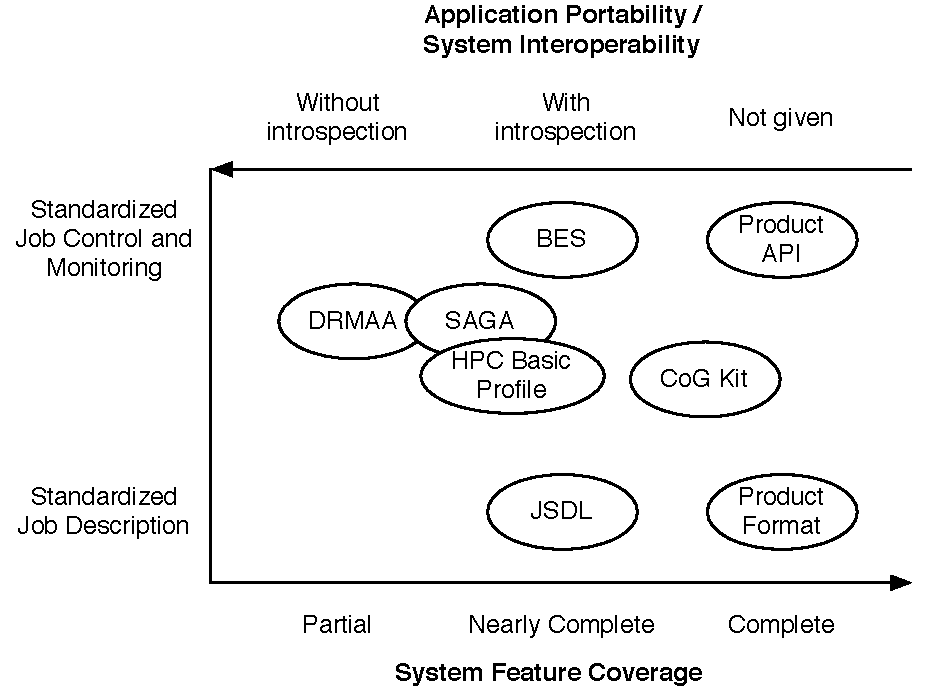
\includegraphics[width=\columnwidth]{hypothesis.pdf}
\caption{Classification of Job Submission and Control Standards for Cluster and Grid Computing}
\label{fig:hypothesis} 
\end{figure}

% AM: CoG Kit?  Is not a standard, but a wrapper around the Globus API versions.
% AM: what is the meaning of the arrow heads?
% AM: A table might be clearer...

%  Standard        Introspection        Feature Completeness
% 
%  Interface Standards
%  DRMAA           no                   partial
%  SAGA            yes                  nearly
%  HPC-BP          yes                  nearly
%  Product API     ?                    complete
%
%  Job Description Standards
%
%  JSDL            yes                  complete
%  DRMAA           no                   partial
%  SAGA            yes                  nearly
%  HPC-BP          yes                  nearly
%  Product Format  ?                    complete

% AM: also: SAGA does not have introspection, DRMAAv.2 does have it.
% SAGA job description is not extensible, DRMAA's is.  DRMAA has more
% DRMS features than SAGA.  So, I think the picture is actually not
% correct?  I do not know if BES and HPC-BP have inspection, and are
% extensible...


\subsection{GLUE}

Beside the role model for this article defined in Section~\ref{sec:rolemodel}, there are other attempts for such a generalization of the stake holders in a \gls{drm} systems. One prominent example is the GLUE specification, which defines a conceptual model for \quote{grid entities} as UML class diagrams. GLUE covers not only the stakeholders defined for this article, but also compute and storage facilities on a fine-grained detail level. A \gls{drm} system is denoted as \emph{Manager} entity in the GLUE context. The execution host concept can be mapped to the idea of an \emph{ExecutionEnvironment} and the \emph{ComputingManager} in GLUE. A job is described as \emph{ComputingActivity}.

% AM: again, I think your 'stakeholders' or 'roles' are 'components' or 'elements'

GLUE in itself is not intended a foundation for technical implementations. It provides a consistent terminology model for varying kinds of batch processing environment, which as the advantage of using precise terminology in the mapping of standards to other environments. 

\subsection{JSDL}

The \gls{jsdl} specification from \gls{ogf} defines a data scheme for job attributes, their inter-relationship and their value range. Job descriptions based on this schema can be re-used in different \gls{drm} systems that support the specification. \gls{jsdl} therefore provides portability for the job description itself, but does explicitely not consider the interfaces for job management and monitoring. Since re-use of job descriptions is one of the primary design goals in \gls{jsdl}, several description properties are limited. One example is the explicitely not supported notion of maximum job run-time, since this is an environment-specific property that cannot be reused.

\gls{jsdl} is a popular and widely accepted format in large-scale \gls{drm} systems. It also helps to implement meta scheduling facilities in grid environments, where job descriptions are forwarded by central management entitity to connected cluster resources. \gls{jsdl} forms one of the cornerstones for HTTP-based job submission and control protocols, such as \gls{wsrf} or \gls{bes}

The specification clarifies how an \emph{extension schema} formulated in XML Schema can be used to create JSDL XML documents that relate to product-specific features and properties. This fulfils the goal of best-possible feature coverage in a standardized document format, while still maintaining some level of job description portability. The implementation of introspection capabilities comes from the usage of XML as description format, which has schema extensibility has inherit concept~\cite{xmlschema}. 

\subsection{BES}

The \gls{bes} specification~\cite{gfd.108} standardized the remote job submission and control through HTTP-based interaction with the \gls{drm} system. Jobs are described through \gls{jsdl} documents. The standard is defining only a minimal set of mandatory operations and job states to be supported by the interface. Beside that, a well-defined extensibility concept allows to add product-specific states and job properties to the interface functionality. 

The BES specification distinguishes between different Web Service port types (see also~\cite{citemaster_579}) for factory operations, activities and management operations. The standard provides a basic state model for activities, which explicitely is intended for being extended by implementations. The idea here is to support ``composable specializations'' based on a common meta model that can support a variety of activities. Examples for from the BES specification are data staging and job suspend operations.

\gls{jsdl} and \gls{bes} were combined into a single set of \gls{drm} system abstractions by the definition of \emph{profiles}, such as the \emph{High Performance Computing (HPC) Basic Profile}~\cite{citemaster_9643}. The profile definition tries to increase the level of interoperability by explicitely restriction some freedom for the implementors, f.e. with respect to the job state model. However, the specification still allows the addition of arbitrary extensions to the \gls{jsdl} job descriptions, while giving the implementation the choice to treat this as an error. Additional efforts in interoperability workshops and tests made BES meanwhile a solid foundation for federated grid environments, as for example with the Unicore middleware~\cite{citemaster_9641}.

\subsection{SAGA}

The \gls{saga} specification~\cite{saga} started as continuation of the \gls{gat} library, a project-specific programming interface for the GridLab middleware~\cite{allen03enabling}. SAGA is an acronym for ``Simple API for Grid Applications'', where ``simple'' is to be understood in the measing of ease of use. Users are intended to be decoupled from the complexities arising in the use of a large-scale distributed system. 

The API is structured into various packages for different purposes, such as logical and physical file management, system management, job management job monitoring, distributed communication and advanced reservation.  Those packages have limited dependencies amongst each other - not all SAGA implementations implement all packages.  All API packages share certain properties: how are synchronous methods expressed, how are notifications realized, how are security tokens expressed, what types of exceptions are defined, etc.  Those properties are specified in the SAGA-Core, the API's look and feel.

That design of the SAGA API allows to specify additional API packages adhering to the same look-and-feel.  In fact, several such API packages have already been defined (e.g., Service Discovery, Messaging etc.), and are standardized as well, or are in the process of being standardized. The interface relies on a consistently asynchronous call model and is described with an IDL-alike syntax.

The SAGA standardization effort is closely synchronized with other specification and community efforts, within and outside of OGF.  In particular, OGF groups ensure that SAGA semantics map well to lover level specifications, such as DRMAA, JSDL, and BES.

The language independent SAGA API specification has been mapped to multiple programming languages, in particular to C++, Java and Python.  Multiple implementations exists, the most notable ones are SAGA-C++, SAGA-Python, JSAGA and JavaSAGA.

SAGA-C++ is, as the name suggests, a C++ implementation of the SAGA API, maintained by LSU and Rutgers University, and a growing international community.  The SAGA-C++ development was in close lockstep with the API specification efforts, and is considered to be complete at this point.

SAGA-Python is a pure Python implementation from Rutgers University, which tries to address several shortcomings of the SAGA-C++ implementation -- it focuses in particular on ease of deployment, small footprint, and code maintenance, and attempts to gather a larger developer community.
  
JSAGA (from IN2P3 in France) and JavaSAGA (from the Vrije Universiteit, Amsterdam) are API compatible Java implementations (they use the same set of abstract class definitions).  JSAGA caters to an active, but small user community in France, and supports a relatively large set of adaptors for the job and file API packages.  JavaSAGA is mostly a academic research vehicle, which bases its middleware bindings mostly on JavaGAT (its predecessor), and sees some uptake in the Netherlands and the German D-Grid project.

SAGA-C++, JSAGA and JavaSAGA all provide python bindings - the Java implementations realize those via Jython, the C++-implementation via Boost-Python.    The Python bindings are thus implemented as a wrappers around the C++ and Java implementations, and are thus able to utilize their complete set of middleware adaptors. The three Python bindings (including the python-native SAGA-Python) are at the moment being unified, and have already been shown to be interoperable.

Interestingly, all SAGA implementations discussed above are adaptor based: a relatively small library provides the SAGA API, and a set of adaptors translate the SAGA API calls into the respective middleware operations.  It is those adaptors which encapsulate most of the complexity which was formerly present in the applications layer.  While SAGA adaptors are relatively easy to implement (at least as a prototype), they require significant maintenance effort to keep up with the middleware intricacies and evolution.

While SAGA is foremost an API, the SAGA distributions support end users in a variety of ways.  In particular, the SAGA distributions also include command line tools implemented via the SAGA API, and higher level libraries for common distributed programming patterns, also basing on the SAGA API.  Further, the SAGA distributions provides comprehensive support to compile, link and run SAGA applications (configure scripts, make support, runtime wrappers, developer tutorials , etc).

Command line tools are, in our experience, amongst the first components of any distributed middleware to be exploited by end users.  Basically all SAGA implementations provide sets of command line tools which cover the important parts of the semantic set of SAGA API calls, such as job submission and management, and file management.

Several SAGA based projects are actively developing and using higher level programming abstractions, such as pilotjobs, bigjobs, mapreduce, or workflows.  Such components are routinely installed and used by a number of user communities, and represent significant added value, although they are not part of the SAGA core code base. 

\subsection{DRMAA}
\label{sec:drmaa}

The \gls{drmaa} specification was designed since the very beginning of grid computing to define a fundamental set of operations for programmatic access to common capabilities of \gls{drm} systems. \gls{drmaa} is focused on the maximum possible level of portability, without disqualify the majority of \gls{drm} systems or the majority of applications. This comparatively harsh restrictions leads to several features intentionally left out, since their semantic either differs between different \gls{drm} systems or because they are not supported by some of the systems. It also marks the primary distinguishing factor between DRMAA und SAGA. While SAGA aims at a high-level, feature complete abstraction of \gls{drm} system functionality, DRMAA aims at the maximum level of portability for applications relying on it. This property makes DRMAA a natural candidate for the implementation of SAGAs job-related functionalities, as shown in Figure~\ref{fig:specstack}. 

\begin{figure}
  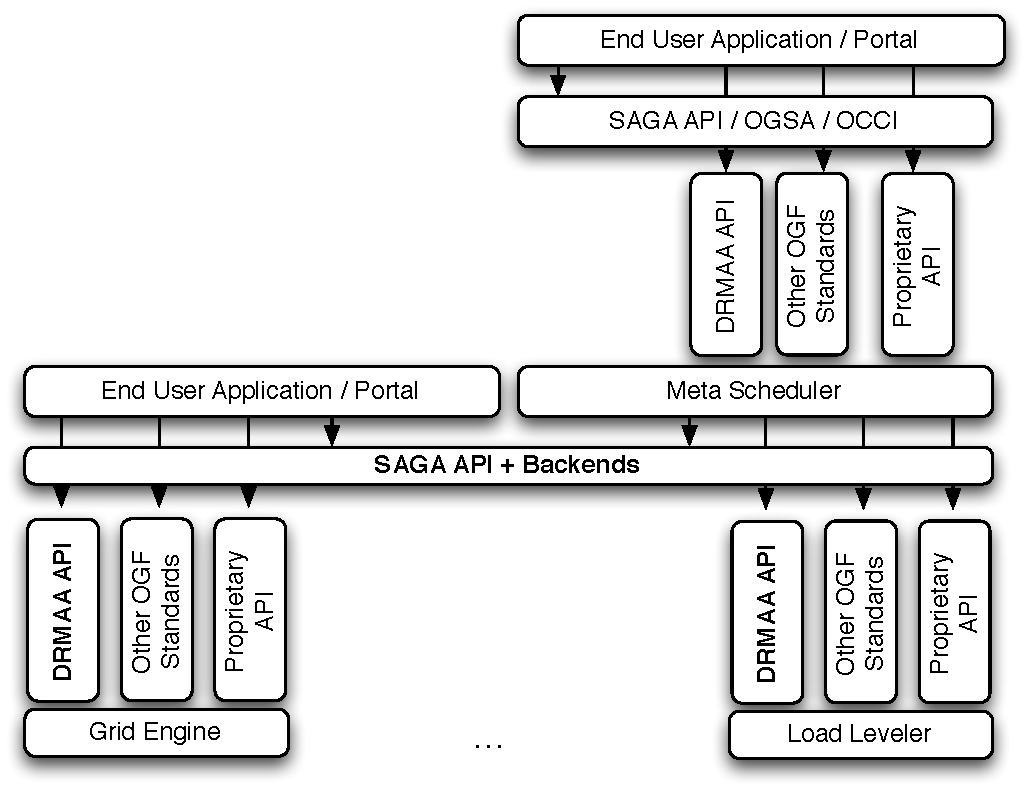
\includegraphics[width=\columnwidth]{specstack.pdf}
\caption{Relation of DRMAA, SAGA, and other OGF specifications}
\label{fig:specstack} 
\end{figure}


Our practical experience in the \gls{drmaa} standardization activity shows that the explicit rejection of API functionality or job information properties is mainly a problem for the implementor side, while the majority of end users does not demand a large set of functionality anyway. Since standardization is also driven by business demands of the participating organizations, it is understandable that vendors want to push their favourite features into the specification.

\gls{drmaa} is intended to be adoptable to multiple programming languages. Similar to other specifications, such as the W3C \gls{dom} specification or SAGA, it relies on the description with a language-agnostic interface description language, in this case CORBA \gls{idl}. Based on a root specification in \gls{idl}, language bindings can map the syntactical constructs to a particular programming language. This leaves the definition of offered functionality, their grouping and the definition of possible error conditions to a single document.

\gls{drmaa} does not consider any security aspect of \gls{drm} systems, since this would demand a choice for platform- or middleware-specific security concept (e.g. Unix UID, X.509, Kerberos). Such a choice would be in contrast to the overall goal of platform independence, portability and simplicity. For this reason, \gls{drmaa} relies on the security context provided with the user running the application. While this seems to be a strong restriction on first look, it acutally serves as crucial precondition for applying DRMAA in environments where authentication and authorization is anyway handled by lower layers. 

The first version of the specification reached the final status of a \emph{grid recommendation} in 2008, with a number of implementations deployed with \gls{drm} systems such as GridEngine, HTCondor, and GridWay. Language bindings and their implementation exist for C, Python, Perl, Java, Ruby, TCL and C\#. 

Due to ongoing development in \gls{drm} system technology, a new version of the \gls{drmaa} specification was published in 2012~\cite{citemaster_9274}. It considers more functionality now common to different \gls{drm} systems and considers also the mapping of DRMAA to a remote usage scenario. The following text refers only to this version of the specification.

DRMAA distinguishes three major classes of functional blocks for job management, advance reservation management and \gls{drm} system monitoring (see Figure~\ref{fig:drmaastack}).

\begin{figure}
  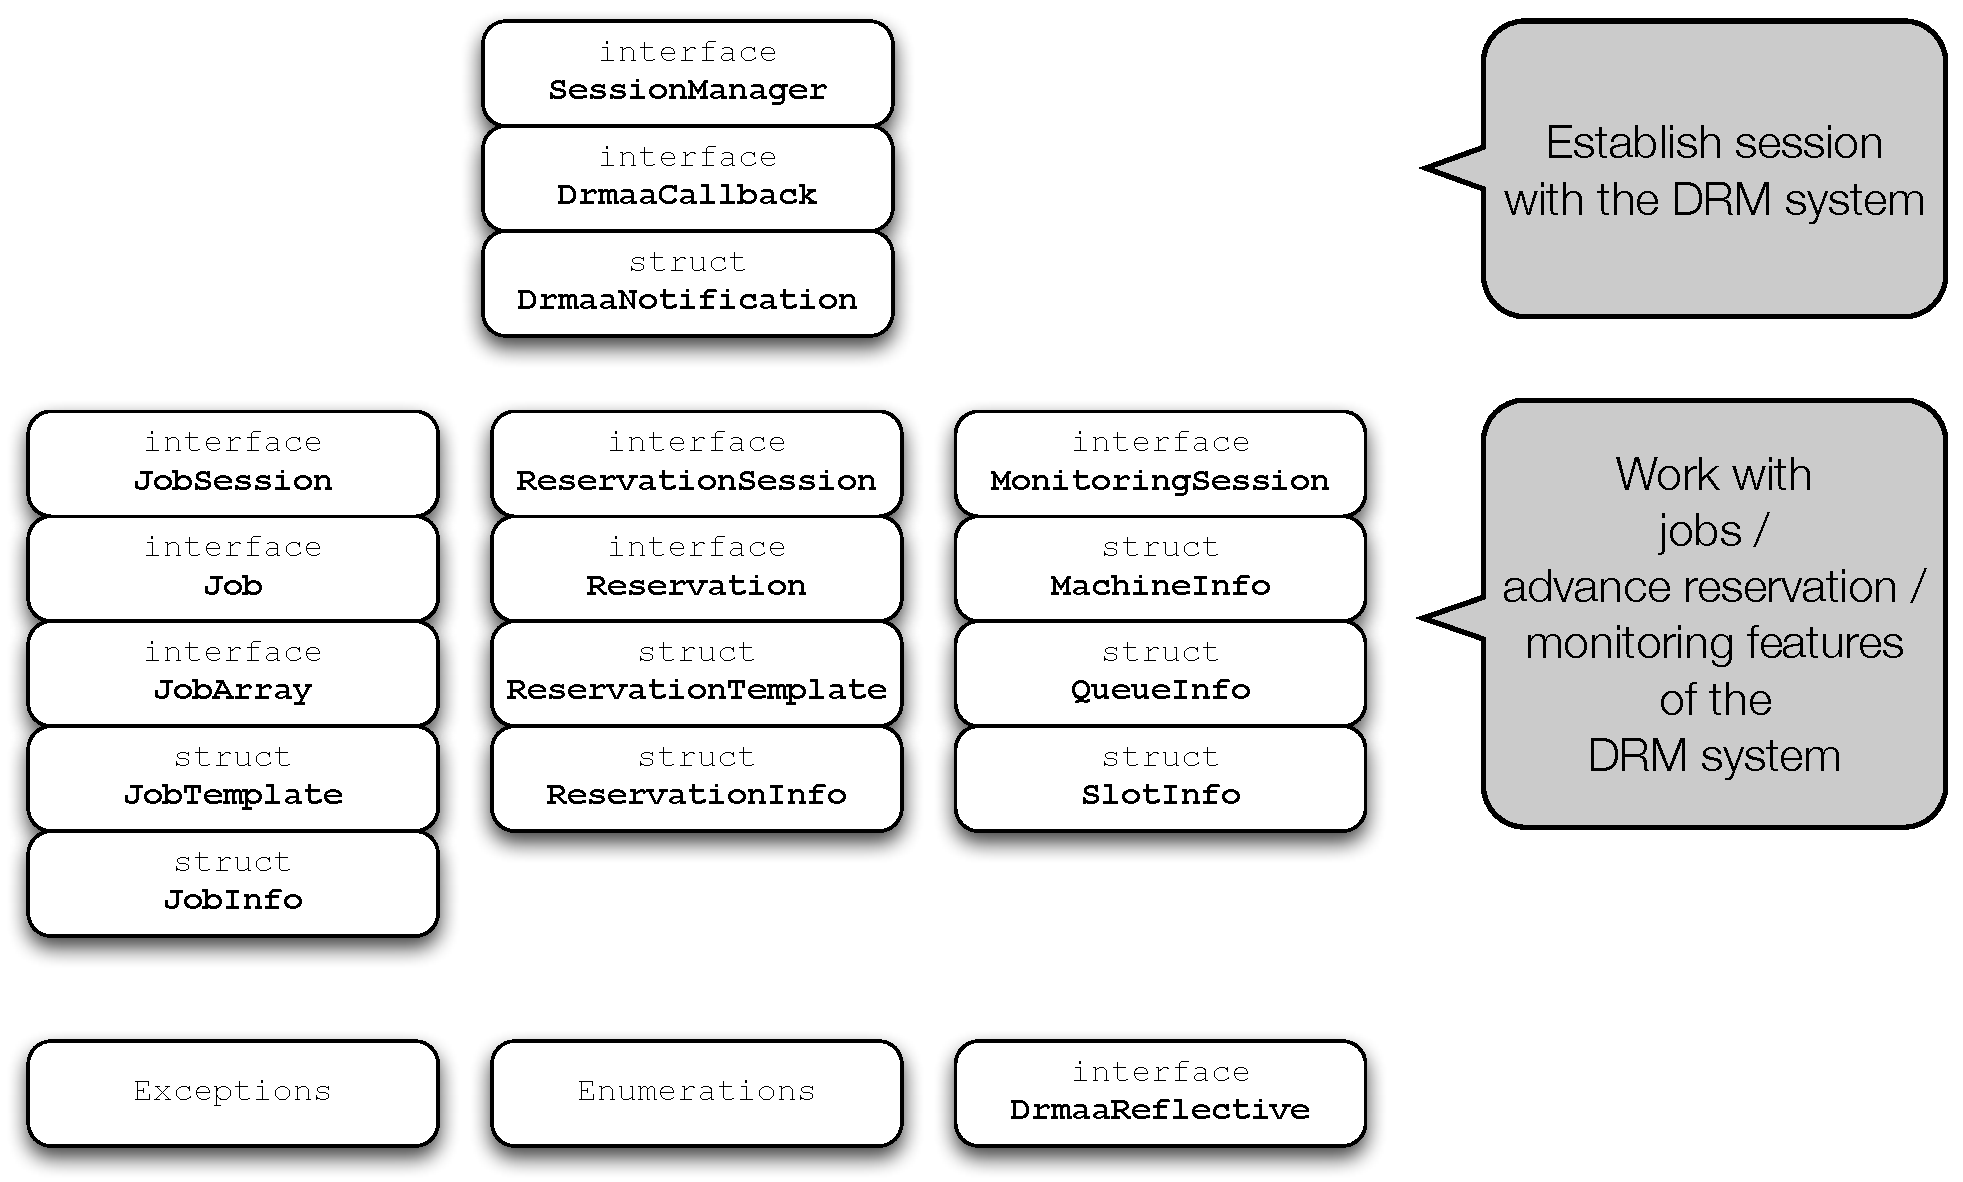
\includegraphics[width=\columnwidth]{drmaastack.pdf}
\caption{Functional blocks in the DRMAA specification}
\label{fig:drmaastack} 
\end{figure}

The specification relies on a session concept to support the persistency of job and advance reservation information in multiple runs of short-lived applications. Typical examples are a job submission portal or command-line tool. The session concept also allows an implementation to perform attach / detach activities with the \gls{drm} system at dedicated points in the application control flow.

The \emph{SessionManager} interface is the main interface of a DRMAA implementation for establishing communication with the \gls{drm} system. By the help of this interface, sessions for job management, monitoring, and/or reservation management can be maintained. Job and reservation sessions maintain persistent state information (about jobs and reservations created) between application runs. The three-fold session concept maps closely to the SAGA API semantics, which ensures that SAGA implementations can easily implement their job-related functionality based on a DRMAA implementation.

The specification mandates the \gls{drm} system itself to persist the neccessary state information until the session is explicitely reaped. If state saving is not possible in the particular \gls{drm} system, then the state data must be persisted in the implementation of the specification (see also Section~\ref{sec:rolemodel}). 

A DRMAA job represents a single computational activity that is executed by the \gls{drm} system. There are three relevant method sets for working with jobs: The \emph{JobSession} interface represents all control and monitoring functions available for jobs. The \emph{Job} interface represents the common control functionality for one existing job. Sets of jobs resulting from a bulk submission are controllable as a whole by the \emph{JobArray} interface. A \emph{ReservationSession} instance acts as container for advance reservations in the DRM system, were each of them is represented by a \emph{Reservation} instance. The \emph{MonitoringSession} interface provides a set of stateless methods for fetching information about the DRM system and the DRMAA implementation itself.

In relation to the dillemma discussion in Section~\ref{sec:hypothesis}, DRMAA makes a set of explicit restrictions in the supported functionality. The majority of functionality must be supported by any implementation, in order to ensure the maximum portability of applications relying on these interfaces. Even then, it was neccessary to have a notion of optional functionality in the DRMAA interface, mainly reasoned by cases where only one, but crucial, \gls{drm} platform was not supporting a particular feature. 

DRMAA solves this by making an explicit distinuishing between \emph{optional} and \emph{implementation-specific} features. Optional features have a clear semantic described by the DRMAA standard. They are part of the interface structures. Any application can programmatically check for the support of a particular optional feature before using it. The concept is similar to the idea of support levels in the POSIX specification series.

The second class of non-mandatory functionality are implementation-specific attributes in data structures. DRMAA only defines how an implementation can add such extensions withouth breaking un-aware applications. This is a similar extensibility approach as with JSDL, BES or any other standard relying on the XML extensibility support. 


\section{Standards for IaaS Cloud Environments}
\label{sec:speciaas}

The previous section discussed established standards for job submission and control in cluster and grid systems.  This section complements that with the state of standardization in IaaS cloud environments, which is equally important for the scope of this article.  

The perceived significance of cloud computing in industry and research projects resulted in numerous standardization activities that are either announced or have started.  One group of cloud standards targets the lifecycle management of service offerings such as virtual machines (IaaS), applications (PaaS) or storage blocks (SaaS). Those standards typically cover the deployment and initialization of new instances, instance management operations, backup operations, bootstrapping support and security.

% AM: SaaS was previously introduced as *Software*aaS, not as *Storage*aaS ...


Another group of standards attempts to unify monitoring functionality -- those standards focus on surveillance and auditing of service-level agreement properties, such as communication latency, throughput or availability.

The third group of specifications focuses on data formats, such as for virtual machines, deployed PaaS applications or application data to be used in a SaaS context. Standards in this group typically relate to lifecycle management specifications from the first group. This relation is comparable to JSDL vs. BES / SAGA / DRMAA development in the grid community - the standardization of description and data formats is separated from, but related to, the API standardization. 

In the context of batch processing interfaces for cloud environments, the first group of specifications is the most relevant, as it applies to infrastructures which are potentially used as \gls{drms} execution resources. Prominent standards from this class are the \gls{occi} specification from the \gls{ogf}, the \gls{ovf} from the \gls{dmtf}~\cite{citemaster_9644}, and the \gls{cdmi} specification from the \gls{snia} standardization body. All three standards have been shown to be combinable to implement a standards-based cloud service offering~\cite{citemaster_9645}. The \gls{ovf} specification defines how a deployment package for IaaS environments can be formulated in a portable way, so that virtual machine configurations are usable with different cloud offerings. \gls{cdmi} offers the means to programmatically manage cloud storage resources. \gls{occi} provides the standardized remote \gls{api} to manage the IaaS resources instances hosted by different cloud providers. It therefore provides the interface to trigger operations on and within the instantiated cloud resources. 

% AM: I am not sure how the statement in the last sentence follows from the previous text -- why is OCCI able to trigger ops *within* instances?

% AM: should we also dedicate a short section to OVF and CDMI?  If not, we need a statement here why not...

\subsection{OCCI}

The \gls{occi} specification is defined as a set of complimentary documents with a core specification~\cite{citemaster_9270}, rendering specifications and extension specifications. The \gls{occi} core specification defines several foundational concepts being used both by \gls{occi} extensions and \gls{occi} renderings:

\begin{itemize}
\item A \emph{resource} is an entity that is exposed through an \gls{occi}-compliant implementation. Extension specification can sub-class the resource type to express specific concepts to be managed, such as virtual machines or storage resources.
\item A \emph{link} entity associates resource entities with each other. One example is the relation between virtual machines and their storage space,
\item Actions and capabilities for resource instances are defined by a \emph{kind} definition. Instances of this type can be linked to resource and link instances, in order to support different activities on the entities.
\end{itemize}

Extension documents can specify resource types, their actions and attributes for a particular application domain of \gls{occi}. Rendering documents specify a wire protocol that represents the OCCI core and extension concepts, f.e. by HTTP verbs and addressable ReST resources~\cite{gfd185}. An example interaction is shown in Figure~\ref{fig:occiexample}, where OCCI is used to instantiate a virtual machine on the cloud provider side.

\begin{figure*}
\begin{lstlisting}
> POST /compute/ HTTP/1.1 
> [...] 
> 
> Category: compute; scheme="http://schemas.ogf.org/occi/infrastructure#"; class="kind"; 
> X-OCCI-Attribute: occi.compute.cores=2
> X-OCCI-Attribute: occi.compute.hostname="foobar" 
> [...]
< HTTP/1.1 201 OK 
< [...] 
< Location: http://example.com/vms/foo/vm1
\end{lstlisting}
\caption{Example: Creating a virtual machine instance}
\label{fig:occiexample} 
\end{figure*}


While the language-agnostic definition of core concepts is similar to the SAGA and DRMAA approach, the extensibility concept is similar to the BES architecture. An \gls{occi} implementation is expected to provide cloud services to a remote client entity as abstraction for the resource management framework on the provider side. Figure~\ref{fig:occiexample} shows an example interaction with OCCI based on the HTTP rendering for the OCCI infrastructure extension~\cite{citemaster_9271}.

\section{Standardized Job Submission in the Cloud}

From the given set of existing cluster and grid standards, BES has a great potential for being used as interoperable interface to batch processing facilities in the cloud. Recent experiments in the \emph{European Middleware Initiative (EMI)} project show how a BES implementation can be deployed inside a virtual machine instance running at the cloud provider side. Another initiative is the HPC Ubercloud Experiment~\cite{citemaster_9647}. The example of BES in the cloud shows an important architectural aspect of batch processing in an IaaS cloud, which we call the \emph{intra-VM} vs. the \emph{inter-VM} approach (see Figure~\ref{fig:vmapproach}).  

\begin{figure}
  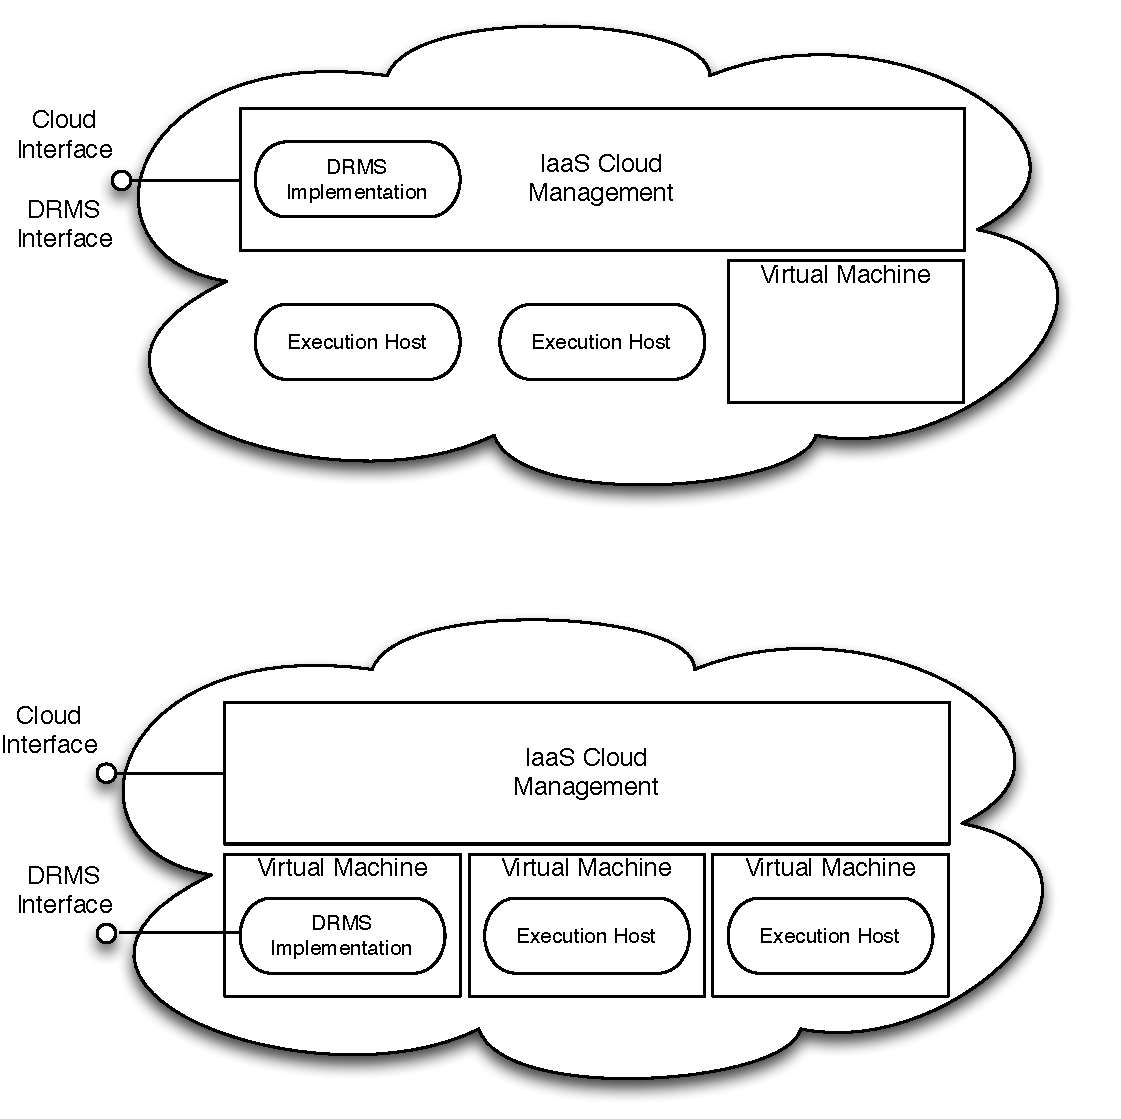
\includegraphics[width=\columnwidth]{cloudapproach.pdf}
\caption{Inter-VM vs. intra-VM approach for batch processing in IaaS clouds}
\label{fig:vmapproach} 
\end{figure}


With the \emph{intra-VM} approach, both the \gls{drm} system and the standardized interface implementation are deployed as part of virtual machines running on cloud resources. This approach makes use of the inherent nature of IaaS offerings, where virtualized resources are used as simple remotely hosted replacement for local execution resources. In theory, it supports the re-use of existing software stacks and standards by just deploying existing middleware stacks in the cloud. This kind of approach is not new - one example from the grid computing field is the Condor GlideIn functionality for extending a Condor pool with resources from a remote Globus installation~\cite{condorgrid}. Practical experience in the grid community showed that this approach, even though it seems to habe a low entrance barrier, suffers from the dynamic nature of remote resources. Virtual machines hosted by an IaaS provider follow the dynamics defined by the operating provider, while most batch processing systems assume dedicated resource ownership for the system where they are installed. This leads to issue with the bootstrapping of cluster installations on cloud resources, the identification of machines, the handling of data traffic between multiple virtual machines. Furthermore, there is now a competition between the virtual machine resource management by the cloud provider and the resource management implemented by the deployed \gls{drm} system.

An alternative approach is the \emph{inter-VM} concept, where the standardized batch processing functionality becomes part of the cloud offering. The job submission and control interface is implemented by the cloud provider, either by the help of the (anyway existing) cloud resource management framework or by the integration of some \gls{drm} system in the cloud infrastructure. Such an offering can be interpreted as SaaS offering, since the provider enables the remote utilization of a new kind of software functionality.

With the given distinuishing between intra-VM and inter-VM solutions, we propose the extension of an existing IaaS cloud standard to support the notion of job batch processing as cloud offering. The idea here is to extend a given cloud interface standard, in this case OCCI, with the \gls{api} concepts known from cluster and grid systems. Our choice here is the DRMAA specification, since it offers the best-possible interoperability in the feature coverage / interoperability tradeoff decision discussed in Section~\ref{sec:hypothesis}. Such an approach allows cloud providers to extend their offerings with a batch processing facility in an \emph{inter-VM} approach.

\subsection{The OCCI-DRMAA approach}
\label{sec:occidrmaa}

The OCCI-DRMAA approach combines the extensibility capability of OCCI with the strict feature set definition given by the the DRMAA specification. It therefore serves both as DRMAA language binding specification and as OCCI extension specification. The behavioral semantic of DRMAA-OCCI actions is taken from the DRMAA specification, while all syntactical aspects of the access protocol are defined by a chosen OCCI rendering.

DRMAA interfaces represent activities on instantiatable entities. They are mostly modeled as OCCI resources:

\begin{itemize}
\item A \emph{drmaa2} resource represents the container for all OCCI-DRMAA resources and the according functionalities. 
\item A \emph{jobsession} resource acts as container for \emph{job} resources and \emph{jobarray} resources. 
\item A \emph{reservationsession} resource acts as container for \emph{reservation} resources. 
\item A \emph{monitoringsession} resource acts as representation of information about the DRM system on provider side. 
\item A OCCI-DRMAA \emph{job} resource represents one job in the underlying DRM system on provider side. Similarly, the \emph{jobarray} resource represents a cluster of jobs.
\item A \emph{reservation} resource represents a successfully created advance reservation in the DRM system.
\end{itemize}

DRMAA IDL interface attributes map to OCCI attributes. The \emph{readonly} modifier for DRMAA attributes translates to the immutability property. The concept of optional or possibly \emph{UNSET} attributes in DRMAA is mapped to a OCCI attribute multiplicity of $0\ldots1$. Id-based or name-based referencing of instances (e.g. of a DRMAA session) is replaced by URI-based referencing.

Original DRMAA methods that return data structure instances are mapped to OCCI or HTTP verb actions that return the location of a new resource instance. By using an appropriate content type in a GET request for such an instance, the client can be even enabled to retrieve a serialized version of the struct instance. Most of the enumeration members from the DRMAA specification, such as for job states, operating system types or quota types, are mapped directly to JSON strings. 

Figure~\ref{fig:getsessions} shows an interaction example for the retrieval of all existing job session through OCCI-DRMAA.

\begin{figure}
\begin{lstlisting}
> GET /drmaa2/jobsession/ HTTP/1.1
> [...]

< HTTP/1.1 200 OK 
< Content-type: text/uri-list
< [...]
< http://example.com/drmaa2/jobsession/17
\end{lstlisting}
\caption{Example: Retrieving all existing job sessions}
\label{fig:getsessions} 
\end{figure}

Figure~\ref{fig:createjob} shows how to establish a job session and submit a job through a OCCI-DRMAA API. In the first step, a job session is created by a POST request. In the second step, a job template resource is created that contains all the relevant job information. With third step, the job execution is implicitely triggered by creating a new \emph{job} resource that refers to the created session and template. The example shows how the abstract concepts from a specification such as DRMAA can be seamlessly mapped to a distributed cloud environment supporting the OCCI specification.

\begin{figure*}
\center
\begin{lstlisting}
> POST /drmaa2/jobsession/ HTTP/1.1
> [...]
> X-OCCI-Attribute: occi.drmaa2.contact="headnode.testbed.platform.com"
> X-OCCI-Attribute: occi.drmaa2.sessionName="MyTestSession"
> [...]
< HTTP/1.1 201 CREATED 
< [...] 
< Location: http://example.com/drmaa2/jobsession/session1
< [...]
> POST /drmaa2/jobtemplate/ HTTP/1.1
> [...]
> X-OCCI-Attribute: occi.drmaa2.remoteCommand="/bin/date"
> X-OCCI-Attribute: occi.drmaa2.machineOS="LINUX"
> X-OCCI-Attribute: occi.drmaa2.email=["peter@troeger.eu","tmetsch@platform.com"]
> X-OCCI-Attribute: occi.drmaa2.emailOnTerminated=true
> [...]
< HTTP/1.1 201 CREATED 
< [...] 
< Location: http://example.com/drmaa2/jobtemplate/template1
< [...]
> POST /drmaa2/job/ HTTP/1.1
> [...]
> X-OCCI-Attribute: occi.drmaa2.session="/drmaa2/jobsession/session1"
> X-OCCI-Attribute: occi.drmaa2.jobTemplate="/drmaa2/jobtemplate/template1"
> [...]
< HTTP/1.1 201 CREATED 
< [...] 
< Location: http://example.com/drmaa2/job/job43
< [...]
\end{lstlisting}
\caption{Example: Creating a job session and submitting a job.}
\label{fig:createjob} 
\end{figure*}

DRMAA interface methods that trigger state changes in the DRM system map to OCCI actions on OCCI resources. DRMAA functionalities that lead to the creation of instances represented by OCCI resources are available as OCCI resource creation activities. DRMAA interface methods that return named instances are not translated to OCCI actions, since this kind of retrieval is possible by formulating a resource location string explicitely. 

DRMAA templates are data structures that express complex information entities as a whole, such as job or advance reservation information. They might be modified by a \gls{drm} system after their creation, which makes them additional OCCI resources without actions.

As discussed in Section~\ref{sec:drmaa}, the DRMAA session concept models the relationship of \emph{Job} and \emph{JobSession} instances. Similarly, it models the relation between \emph{Reservation} and \emph{ReservationSession} instances. In OCCI-DRMAA, these relationships are represented by OCCI links between the according resource entities -  a \emph{joblink} resource represents the connection of a job to it's job session, and a \emph{reservationlink} resource represents the connection of an advance reservation to it's reservation session.

DRMAA also defines a set of exceptions that may be thrown by API activities. In OCCI-DRMAA, the mapping of these exceptions depends on the chosen transport rendering. This demands the specification of exception mappings to a particular rendering method, as for example shown in Table~\ref{tab:exceptions}.


\begin{table}[ht]
\centering
\begin{tabularx}{\columnwidth}{|l|>{\raggedright\arraybackslash}X|}
\hline
DRMAA Exception & HTTP Error Code\\
\hline
DeniedByDrmsException & 401 / 403 \\
DrmCommunicationException & 500 \\
TryLaterException & 503, with retry header \\
TimeoutException & 410 \\
InternalException & 500 \\
InvalidArgumentException & 400 \\
InvalidSessionException & 404 \\
InvalidStateException & 409 \\
OutOfResourceException & 503, without retry header \\
UnsupportedAttributeException & 400 \\
UnsupportedOperationException & 405 \\
ImplementationSpecificException & 500 \\
\hline
\end{tabularx}
\caption{Mapping of DRMAA exceptions to HTTP error codes.}
\label{tab:exceptions}
\end{table}

As all \gls{api}s initially intended for local library implementations, DRMAA supports the notion of blocking status wait calls for both the \emph{Job} and the \emph{JobSession} interface. Our OCCI-DRMAA approach therefore re-models synchronous calls with the concept of a wait handle URI. An example can be seen in Figure~\ref{fig:waitjobstart}.

\begin{figure*}
\begin{lstlisting}
> GET /drmaa2/job/job43?action=waitstarted HTTP/1.1
> [...] 
> X-OCCI-Attribute: occi.drmaa2.timeout="..."
> [...] 

< HTTP/1.1 202 ACCEPTED
< [...] 
< Location: /drmaa2/job/job43/waithandle1
< [...] 

> GET /drmaa2/job/job43/waithandle1 HTTP/1.1
> [...] 
< HTTP/1.1 404 NOT FOUND

> GET /drmaa2/job/job43/waithandle1 HTTP/1.1
> [...] 
< HTTP/1.1 410 GONE

> GET /drmaa2/job/job43/waithandle1 HTTP/1.1
> [...] 
< HTTP/1.1 301 MOVED PERMANENTLY
< [...] 
< Location: /drmaa2/job/job43
< [...] 
\end{lstlisting}
\caption{Waiting for job start in OCCI-DRMAA}
\label{fig:waitjobstart} 
\end{figure*}

The wait action returns the location of the wait handle, which can be further used for polling GET requests to the server. The server must then return one of these three possible error codes on such request:

\begin{itemize}
\item \emph{Still waiting} (HTTP error 404): The blocking wait call is still running, no timeout occurred so far. The wait handle location remains valid.
\item \emph{Timeout} (HTTP error 410): The blocking call was terminated due to timeout. The wait handle location is now invalid.
\item \emph{Success} (HTTP error 301): The blocking call was terminated since the wait condition was fulfilled. The wait handle location is now invalid.
\end{itemize}

The DRMAA API does not specifically assume the existence of a particular security infrastructure in the DRM system. It is assumed that credentials owned by the application using the API are in effect for the DRMAA implementation too, so that it acts as stakeholder for the application. This relays the responsibility of authentication to the OCCI rendering specification that is used to realize the wire protocol of an implementation. 

\section{Summary}

\printglossaries

\bibliography{citemaster}

\end{document}

